\documentclass[../report.tex]{subfiles}

\begin{document}

In dit hoofdstuk wordt het gerealiseerde project met alle deelproducten besproken en wordt er uitgelegd waarom bepaalde keuzes zijn gemaakt. De broncode van de programma's is bijgevoegd in het portfolio.

\section{De OpenAPI-specificatie}

De \gls*{OpenAPI-specificatie} is een specificatie voor het beschrijven van de \gls*{REST} \gls*{API}. Er is gekozen om hiervan gebruik te maken omdat het als referentie voor communicatie tussen de verschillende deelproducten dient, en omdat er code mee gegenereerd kan worden. Als er wijzigingen zijn aan de specificaties die verzameld moeten worden, kunnen programma's moeiteloos aangepast worden door de \gls*{OpenAPI-specificatie} aan te passen en code te hergenereren.

De \gls*{OpenAPI-specificatie} wordt gebruikt door alle andere deelproducten. In onderstaande kopjes wordt dit per project toegelicht.

\section{ssot-specs-server}

\begin{figure}[ht]
  \centering
  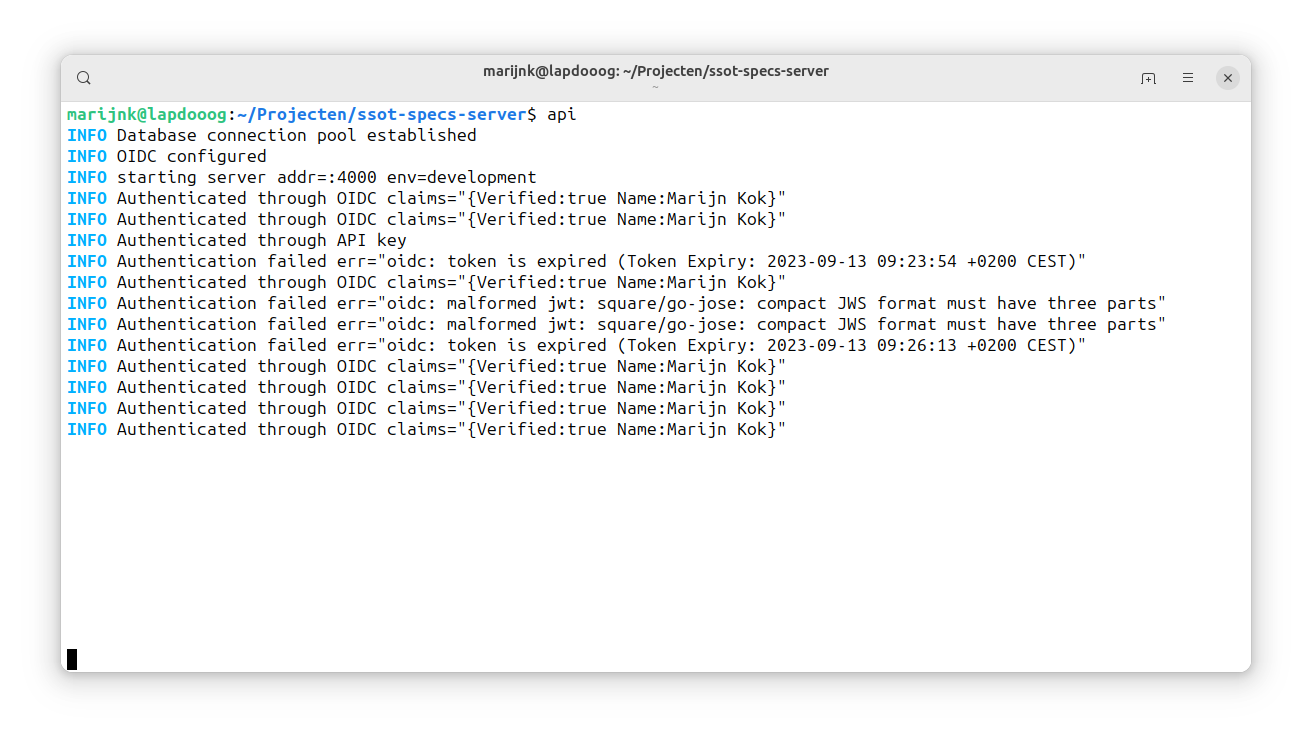
\includegraphics[width=0.85\textwidth]{assets/images/ssot-specs-server.png}
  \caption{Screenshot van een terminalvenster waarin de server wordt uitgevoerd.}
  \label{fig:api_screenshot}
\end{figure}

De server is het middelpunt van het project. Het is een \gls*{REST}ful \gls*{API} die de specificaties opslaat en beschikbaar stelt. Het is geschreven in \gls*{Go} omdat het goede performance biedt en reeds binnen Voys gebruikt wordt. Zo kan het project beheerd, gereviewt en bijgewerkt worden door andere ontwikkelaars bij Voys. Bovendien is er reeds ondersteuning voor de taal, bijvoorbeeld met packaging en \gls*{CI/CD} pipelines. Een screenshot van het draaiende programma is te zien in \autoref{fig:api_screenshot}.

Om gegevens op te slaan wordt gebruik gemaakt van de GORM-bibliotheek\footnote{\url{https://gorm.io}}. Dit is een \gls*{ORM}, wat betekent dat het een abstractie biedt over de database. Dit verkleint de kans op SQL-injecties aanzienlijk en maakt het ontwikkelproces gemakkelijker. Het maakt ook automatische databasemigraties mogelijk. Evengoed had de ingebouwde SQL-bibliotheek gebruikt kunnen worden, maar deze biedt geen automatische migraties en vereist dat SQL-queries handmatig worden geschreven.

Voor authenticatie is gekozen voor \glspl*{API-sleutel} en OpenID Connect (\gls*{OIDC}). Er is voor \gls*{OIDC} gekozen omdat de \gls*{API} dan geen gebruikersgegevens hoeft op te slaan; dit vermindert het aanvalsoppervlak. Bovendien hoeven gebruikers geen nieuw account te maken. De collector gebruikt de \gls*{API-sleutel} om gegevens te sturen. Hiervoor is gekozen omdat collectors zonder gebruikersinterventie moeten werken, en het gebruik van \gls*{OIDC} op eindgebruikers gericht is.

De \gls*{server} had eveneens met de \gls*{OpenAPI} Generator kunnen worden gegenereerd. Er is desondanks niet voor deze aanpak gekozen omdat het slechts een deel genereert en niet aansluit op het gebruikte boek \textit{Lets Go Further}.

\section{ssot-specs-collector}

\begin{figure}[ht]
  \centering
  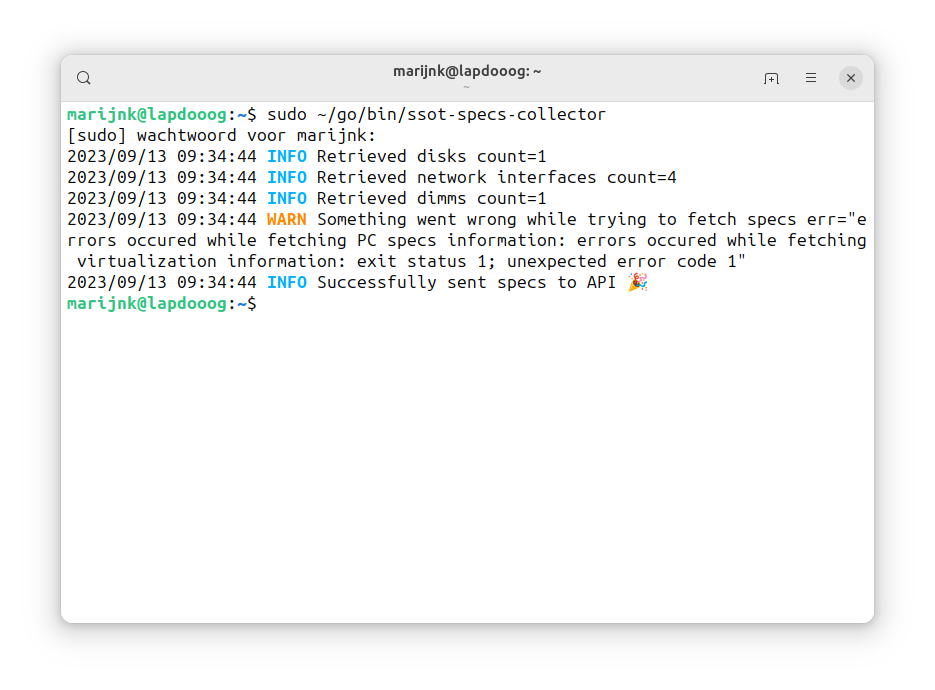
\includegraphics[width=0.85\textwidth]{assets/images/ssot-specs-collector.png}
  \caption{Screenshot van een terminalvenster waarin de collector is uitgevoerd.}
  \label{fig:collector_screenshot}
\end{figure}

De collector verzamelt statische informatie over het apparaat waar het op uitgevoerd wordt, zoals gedemonstreerd wordt in \autoref{fig:collector_screenshot}. Vervolgens stuurt het deze informatie naar de \gls*{API}. Dit gebeurt met behulp van een bibliotheek die gegenereerd wordt met de \gls*{OpenAPI} Generator. De verzamelaar is net zoals de \gls*{API} geschreven in \gls*{Go}.

De gegevens van het apparaat worden verzameld met behulp van verscheidene \gls*{Go}-bibliotheken. Als alternatief had gebruik gemaakt kunnen worden van shell scripts, zoals het programma GoCollect doet \parencite{gocollect}. Er had zelfs gekozen kunnen worden om de collector helemaal niet te schrijven, en in plaats daarvan GoCollect te gebruiken. De keuze is gemaakt om dit niet te doen omdat GoCollect veel onnodige functionaliteit heeft. Bovendien maakt het gebruik van shell scripts het programma platformafhankelijk, terwijl bibliotheken vaak meerdere besturingssystemen ondersteunen. De opdrachtgever heeft echter geen interesse getoond in het gebruik van besturingssystemen die niet de Linux-kernel gebruiken.

\section{infra-ssot-dashboard}

\begin{figure}[ht]
  \centering
  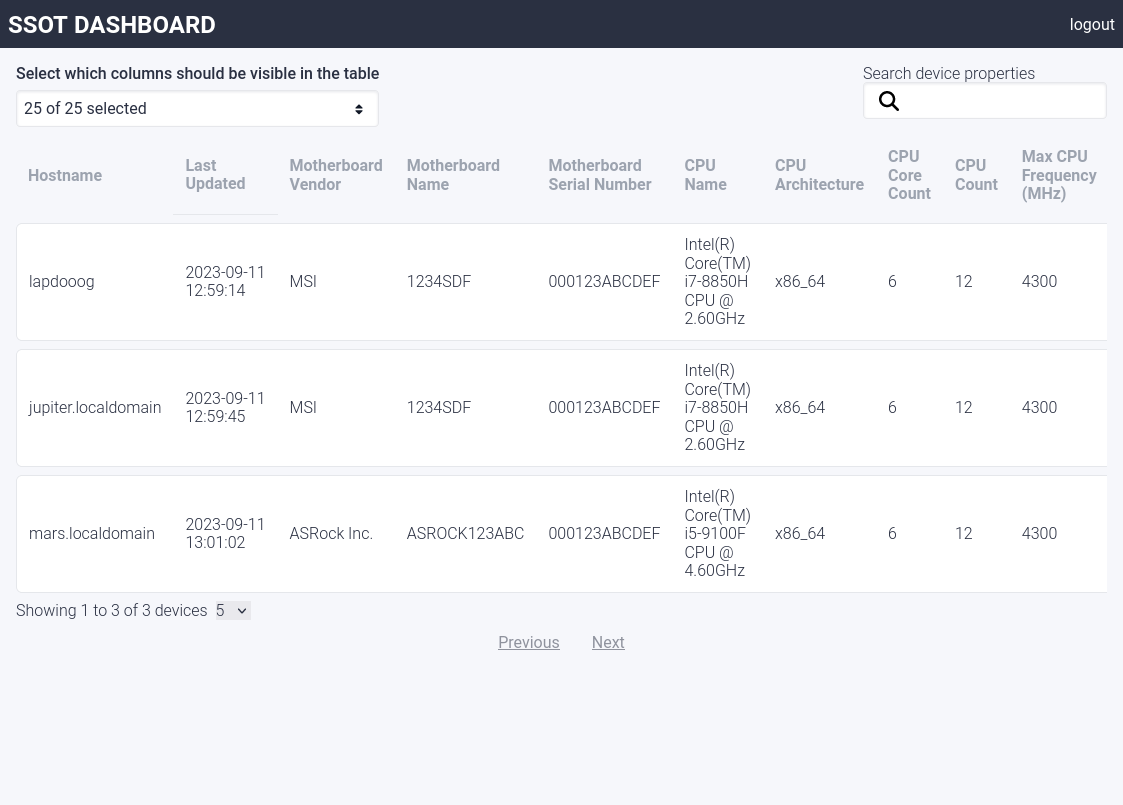
\includegraphics[width=0.85\textwidth]{assets/images/infra-ssot-dashboard-table.png}
  \caption{Screenshot van het dashboard, met drie demo-apparaten. De tabelweergave is horizontaal scrollbaar.}
  \label{fig:dashboard_screenshot_table}
\end{figure}

\begin{figure}[ht]
  \centering
  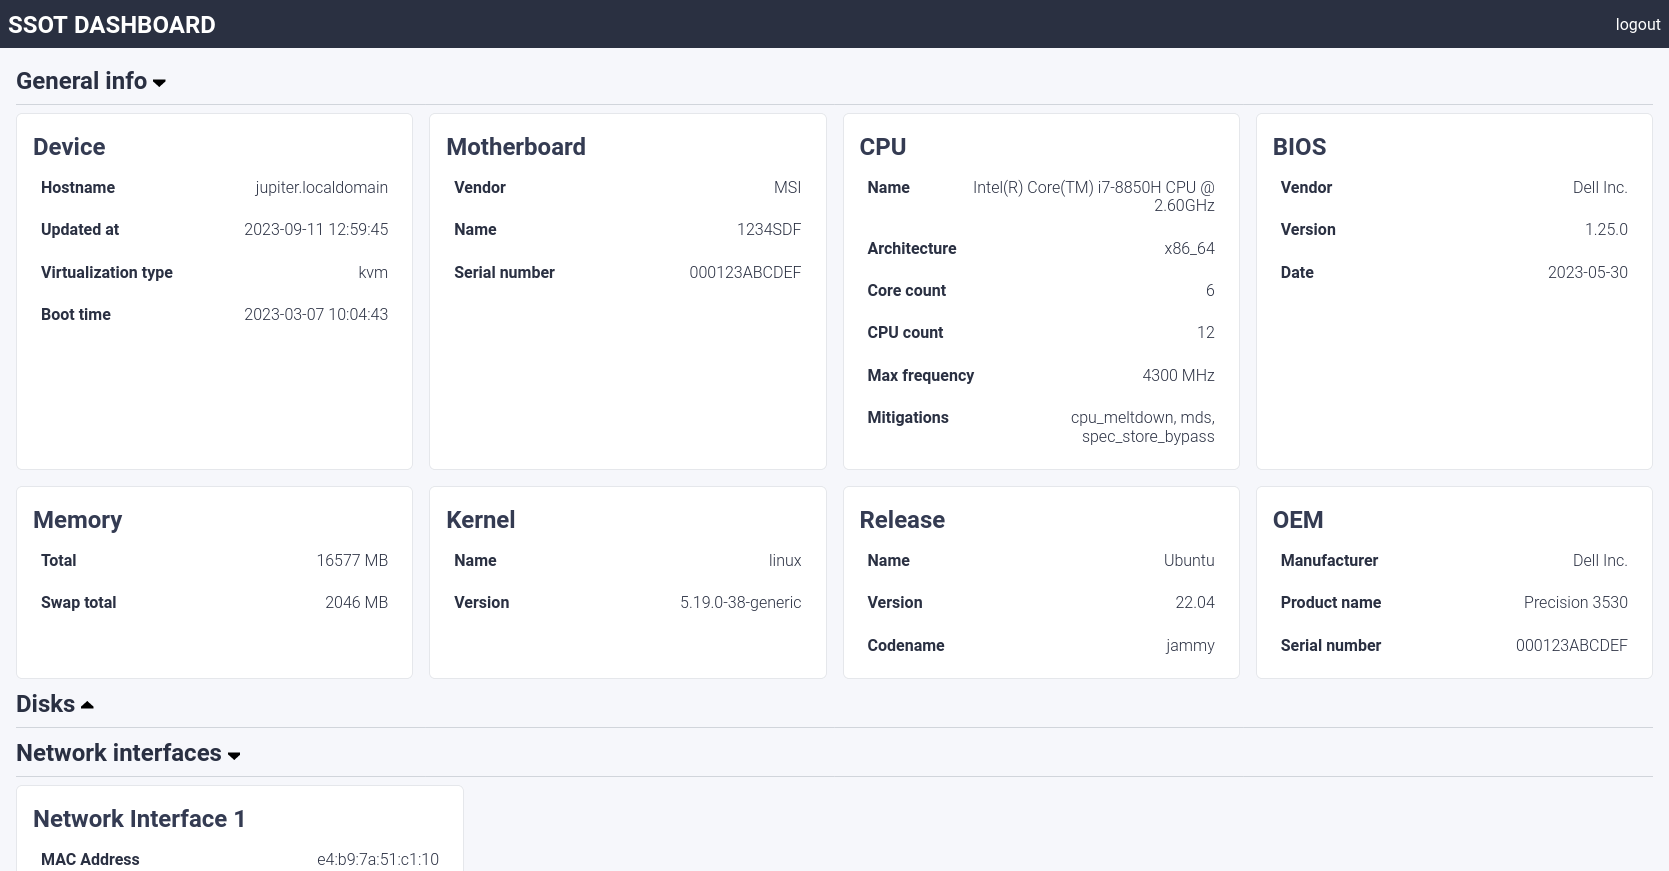
\includegraphics[width=0.85\textwidth]{assets/images/infra-ssot-dashboard-details.png}
  \caption{Detailpagina van een apparaat. De sectie met schijven is dichtgeklapt.}
  \label{fig:dashboard_screenshot_details}
\end{figure}

Het dashboard is een webapplicatie die de specificaties van de apparaten in tabel- of overzichtsweergave toont uit de \gls*{API}. Twee screenshots van de applicatie zijn te zien in \autoref{fig:dashboard_screenshot_table} en \ref{fig:dashboard_screenshot_details}. Het is geschreven in TypeScript en gebruikt \gls*{Preact} en \gls*{Tailwinds}. Hiervoor is gekozen omdat dit reeds binnen Voys gebruikt wordt. Bovendien lijkt \gls*{Preact} op het populaire framework React, maar is het slechts 3kB groot \parencite{preact}.

Bij dit project is er potentie om gebruik te maken van codegeneratie, zoals ook bij de collector gebruikt wordt. Er zijn maar liefst elf opties voor het genereren van typescript code beschikbaar \parencite{openapi_generator}. Er is echter niet voor gekozen om dit te doen omdat het niet goed aansluit bij bibliotheken van Voys. Er is echter een middenweg gevonden om toch code te kunnen genereren met behulp van een externe website\footnote{\url{https://transform.tools/json-to-typescript}}.

\section{4+1 model}

Het 4+1 model is een model voor het beschrijven van de architectuur van een softwareproject. Het model bestaat uit vijf ``views'': logical, process, development, physical en scenario. Alle 4+1 model-views van de collector, server en het dashboard zijn te vinden in de bijlage \parencite{four_plus_one_model}.

% \section{Slot}

% Al deze programma's werken samen om het project te realiseren. De collector stuurt gegevens van een computer naar de \gls*{API}, en deze slaat ze op. De webapplicatie vraagt de gegevens van de \gls*{API} om ze weer te geven. Maar code is niet het volledige plaatje. Er is ook een infrastructuur nodig om de programma's op te draaien. Hoe de code draait op de infrastructuur wordt in het volgende hoofdstuk besproken.

\end{document}
